%!TEX root = project.tex

\chapter*{About this project}
% assuming past tense as this report is talking about the completed project
\paragraph{Abstract}
%A brief description of what the project is, in about two-hundred and fifty words.
% leave technical jargon out of it
This project sets out to create a food ordering system for a local company. 
The systems primary components are a mobile application that the user interacts with and a web application that the staff interact with.

The need for such a system stems from two problems, firstly the issue of rush hour times during business hours where there is a vast number of customers to service, and secondly to bring more presence and promotion to the business, as they are finding it hard to reach out to their current customer base and would be customers.

% Mobile app
We aim to solve the first problem by having a system in which customers can pre-order sandwiches and other products via a mobile application.
Users will be able to top up their account, order products, pick a collection time, and view their balance, products and past order history.

The second problem will be solved by implementing push notifications into the application so that the company can let customers know about menus, events and various other updates. Another way to increase promotion and presence is by having various information about the company on the application; for instance: opening times, contact details and general information. 

% web app
All of the information on the web application can be updated; this includes the menus, opening times, user and staff details, and much more. 
This information is reflected in the web application.
Interactions from within the mobile application including: topping up, logging in, registration and ordering go through the web application.

% conclusion
We plan to create a cohesive, thoughtfully designed, robust system that solves these two problems.
\pagebreak

\paragraph{Authors}
%Explain here who the authors are.
This project was created by two fourth year software development students: Ronan Connolly \& Vladislav Marisevs, as part of our Bachelors of Science honours degree in Software Development. 
\linebreak

Ronan was in charge of creating all aspects of the user facing mobile app. 
Vladislav was in charge of creating all aspects of the staff facing web app.
\linebreak

We spent most of our shared time coming up with the overall architecture we would implement, and an interface to be used between mobile and web app for transfer of data.


\pagebreak
\paragraph{Acknowledgements}
We would like to acknowledge and thank our supervisor Dr John Healy for all the time and effort he has put into helping us throughout this project, he gave us a good structure and set milestones for us in order to keep on top of things.
\linebreak

We'd also like to thank the GMIT Catering Company staff for the time spent meeting with us in order to continuously improve and adapt the project.

\chapter{Introduction}	% 3-5 pages
%The introduction should be about three to five pages long.
%Make sure you use references~\cite{einstein}

% should contain a breif intro the the project, how it came about, the reason for it.
% also will break it down into an intro to the latter chapter?

% abstract (change)

%% CONTEXT
% basic idea
We set out to create a food ordering system for the GMIT Catering Company (known henceforth as the company).
The basic structure is a mobile application (henceforth known as mobile app) for the Android and iOS systems that the user interacts with, and a server (henceforth known as web app) that the staff can log into in order to view transactions, user details and to update the mobile app.

% reason #1
The reason such a system is needed is that queues during peak times tend to be enormous and currently it's hard to service all the customers.

% reason #2
Another reason is to encourage customers to get into a habit of repeat ordering, if it is an easy process then it should increase purchases.

% reason #3
Lastly, the company wants to increase presence and promotion in the college, in order to achieve this end we have implemented push notifications where staff can send a notification to all users. On top of this the mobile application itself serves as a promotional device, containing details of various aspects of the company.
\linebreak

%% OBJECTIVES
% mobile app features
The components contained within the mobile app include pages for login, registration, about the company and user details There is also a way to top up and order sandwiches.
A huge emphasis is put on design for this project, using the companies colour theme and creating a nice icon.
% tech
This mobile app was created using the Ionic Framework which is programmed primarily using the AngularJS framework.

% web app features
The components contained within the web app include many pages such as the login system, orders, stock, user details, vouchers(for adding credit to your account), settings(collection and opening times) and accounts(staff) pages.
%tech
This web app was created in PHP using Zend Framework 2.
% reflection in app
Most of the information on the web app is reflected on the mobile app.

% connect the apps
The two applications talk to each other via JSON over HTTP Get and Post requests. 

% conclusion
We set out to create a well thought out, carefully designed, robust food ordering system using modern technologies.
This project could be extended in the future to be used 
\linebreak

% authors (change)
% mention how to laid it out between us
% We thought out, designed and carefully laid out this project into many smaller components.
%Ronan was in charge of creating all aspects of the user facing mobile app. 
%Vladislav was in charge of creating all aspects of the staff facing web app.


% mention agile
We used an agile structure where we had certain components we needed complete by specific dates.
% mention meetings
We had various meetings each month with our supervisor and several members of the company.

%% CHAPTER SUMMARIES


%% GITHUB URLS
%% Web App

%% Mobile App

% main link

% test server link

% push link

\chapter{Context}	% 3-5 pages
\begin{itemize}
\item Our project consists of creating a food ordering system for the GMIT Catering Company.
\item Our basic objectices were to create a mobile and web application to deal with the above item.
\end{itemize}

Below we will:
\begin{itemize}
\item list what each chapter contains below.
\item list out the various elements in our Github repositories below.
\item explain the various components of our project.
\end{itemize}

\section{Web App}

I decided to do this because of that, etc
PHP is great but maybe a Java web server would have being better, easier to modify, I already know Java.
SQL is hard to change over time, maybe implementing a NoSQL database would have been good...

\section{Mobile App}
The mobile application is created using bleeding edge technologies such as the Ionic framework, which utilizes the AngularMVW framework, which in turn is programmed using JavaScript. HTML and CSS were also heavily utilized.

Initially I had no idea about JavaScript, web development or cross platform development. I spent much time studying JavaScript, Angular, Ionic, and the MEAN Stack (MongoDB, ExpressJS, AngularJS, and NodeJS). I then spent a lot fo time trying out various cross platform development frameworks.

I will speak more in detail about these technologies in the technology review chapter.

\subsection{Cross Platform Frameworks}

I first tried out Cordova, which I found had the capabilities to do pretty much anything, but the community and framework is very sparse, it's hard to get anything up and running, and the stylings are horrid.
\cite{https://cordova.apache.org/}

Next I tried out JQeuryMobile which had better styling but again I came across many issues.
\cite{http://jquerymobile.com/}

Finally I came across the Ionic Framework which uses Cordova underneath. This framework has a huge community of developers, it has the support of Google, Microsoft and many other large companies. They closely work with the Angular team at Google and the TypeScript team at Microsoft. 
They have a 24/7 group chat system set up with various sub rooms. 
They have amazing documentation, regular blog posts, quick response to questions on the blog, forums and chat. 
With Ionic you get:
\begin{itemize}
\item All the capabilities of Cordova, which allows you to access the Mobiles native APIs easily
\item A slick native UI experience. The app changes design depending on the platform it's running on
\item Extensive tooling. Starting an app, templates, app store image creation, logo creator, etc
\item Rapid development cycle, there are constant updates (which can cause issues, but is usually great)
\end{itemize}
\cite{http://ionicframework.com/}

\subsection{Tooling}
Once I decided on using the Ionic framework I spent my time completing various JavaScript, Angular and Ionic tutorials. This was a steep learning curve as there is so much tooling for all the JavaScript frameworks.
I installed NodeJS in order to use NPM (Node Package Manager) in order install Ionic. 

Then Ionic came with it's own tools for various tasks, including SASS for programmatic CSS, Bower (Like NPM or Maven) for adding in new components, Grunt for running tasks (like Ant) and some others like Gulp (similar again to NPM).

Each of these tools takes time to learn. I read documentation and completed at least one tutorial for each.

\section{Push Server}
In order to facilitate push notifications I needed to get their device token and save it in a database.
I created a controller in the mobile application, once the app starts it gets the device token along with some other information and sends it to the push server.

The push server is always listening for incoming requests, once it receives one it evaluates it, adds a timestamp and saves the user object (JSON) to a CouchDB server (Using IBM's Cloudant Web Server).

The push server is a MEAN Stack, Yeoman scafolded project that uses NodeJS as the environment, Express as the Web Framework and Angular as the MVC (Model View Controller) framework in order to build the web application.
\linebreak

The reasons we chose to have the push notification server separate is that:
\begin{itemize}
\item We did not realise we needed to save the device tokens initially and to implement this new table into the SQL schema is a big effort
\item We wanted to try out a MEAN Stack application
\item We felt there was no big dissadvantage on having the push server seperate
\item The mobile app is so tightly integrated with the push server (everything is written in JavaScript), that it made creating the web application extremely simple
\item The GMIT Catering company may assign the task of push notifications to somebody that they do not wish to have access to the food ordering system, such as a social media expert. 
\end{itemize}

Users can:
\begin{itemize}
\item Login/Logout via username and password
\item View how many devices are registered for push notifications
\item View previously sent push notifications
\item Send new push notifications, and see if they were sent successfully.
\end{itemize}


\chapter{Methodology}	% 1-2 pages
About one to two Pages

Describe the way you went about your project:
\begin{itemize}
\item We used an Agile / incremental and iterative approach to development. 
\item There were plently of meeting and planning with our supervisor and the companies manager.
\item We did user testing on the app, and constantly made sure all the routes were working.
\item We designed a RESTful style route interface. This let us work on our own components without the web and mobile app waiting for each other.
\item We used Github during the development process, tracking tasks via the Github Issue tracker.
\item We tested out various technologies at each step of the way and discussed why we were choosing each one.
\end{itemize}

Check out the nice graphs in Figure \ref{tikz:graphs}, and the nice diagram in Figure \ref{tikz:mydiagram}.

\begin{figure}
	\centering
	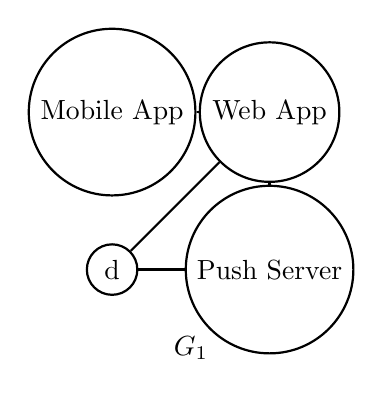
\begin{tikzpicture}
	\begin{scope}[every node/.style={circle,thick,draw}]
	\node (a) at (0,2) {Mobile App};
	\node (b) at (2,2) {Web App};
	\node (c) at (2,0) {Push Server};
	\node (d) at (0,0) {d};
	\end{scope}
	\begin{scope}[every edge/.style={draw=black,thick}]
	\path (a) edge (b);
	\path (b) edge (c);
	\path (b) edge (d);
	\path (c) edge (d);
	\end{scope}
	\node () at (1,-1) {$G_1$};
	\end{tikzpicture}
	\hspace{1.5cm}
	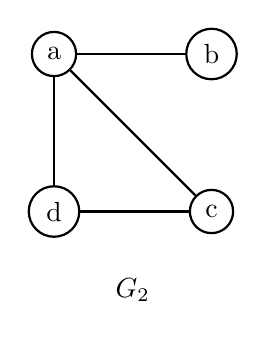
\begin{tikzpicture}
	\begin{scope}[every node/.style={circle,thick,draw}]
	\node (1) at (0,2) {a};
	\node (2) at (2,2) {b};
	\node (3) at (2,0) {c};
	\node (4) at (0,0) {d};
	\end{scope}
	\begin{scope}[every edge/.style={draw=black,thick}]
	\path (1) edge (2);
	\path (1) edge (3);
	\path (1) edge (4);
	\path (3) edge (4);
	\end{scope}
	\node () at (1,-1) {$G_2$};
	\end{tikzpicture}
	\caption{Nice pictures}
	\label{tikz:graphs}
\end{figure}

\begin{figure}
	\centering
	\begin{tikzpicture}[node distance=6cm]
%	\node (a) [rect] {A Big Blue Block};
%	\node[rect](name)
	\node (a) at (4,2) [draw,thick,minimum width=2cm,minimum height=2cm, blue] {A Big Blue Block};
	\node (b) [oval, right of=a] {And His Oval Friend};
	\draw [line] (a) -- (b);
	\end{tikzpicture}
	\caption{Nice pictures}
	\label{tikz:graphs}
\end{figure}


\chapter{Technology Review}	% 7-10 pages
About seven to ten pages.
\begin{itemize}
\item Describe each of the technologies you used at a conceptual level. Standards, Database Model (e.g. MongoDB, CouchDB), XMl, WSDL, JSON, JAXP.
\item Use references (IEEE format, e.g. [1]), Books, Papers, URLs (timestamp) – sources should be authoritative. 
\end{itemize}

\section{Web App}	% 4 pages
I decided to use PHP since I was already proficient at it and it works really well as a web app because....

\subsection{PHP}

\subsection{Zend Framework}

\pagebreak

\section{Mobile App} % 4 pages
\subsection{Ionic Framework}
% talk about JS, AngularJS, CSS, HTML and Ionic.
\subsubsection{HTML/CSS}

\subsubsection{JavaScript}

\subsubsection{AngularJS}

% Here's some nicely formatted XML:
% \begin{minted}{xml}
% 	<this>
% 	<looks lookswhat="good">
% 	Good
% 	</looks>
% 	</this>
% \end{minted}

\subsection{Tools}
\subsubsection{Yeoman}

\subsubsection{Grunt}

\subsubsection{Jasmine}

\subsubsection{Jade}

\subsubsection{Bower}

\subsubsection{NPM}

\subsubsection{BASH}

\subsection{Alternatives}
% alternatives? JQueryPhone, PhoneGap, Cordova, Xamarin
\subsubsection{Cordova}

\subsubsection{PhoneGap}

\subsubsection{JQueryMobile}

\subsubsection{Xamarin}

\section{Push Server}


\subsection{CouchDB/Cloudant}

\subsection{NodeJS}

\subsection{ExpressJS}


\section{REST Architecture}	% 1/2 pages
\subsection{HTTP Requests}
% talk about the HTTP get/post requests used via the interface from the phone and server
\subsection{Custom API}
% The web server has a custom API that the mobile app uses

\section{JSON}	% 1 pages

\chapter{System Design}	% n-m pages
As many pages as needed.
\begin{itemize}
\item Architecture, UML etc. An overview of the different components of the system. Diagrams etc… Screen shots etc.
\end{itemize}

\begin{table}[h]
  \centering
  \begin{tabular}{x{2cm}p{3cm}}
    \toprule \\
    Column 1 & Column 2 \\
    \midrule \\
    Rows 2.1 & Row 2.2 \\
    \bottomrule
  \end{tabular}
  \caption{A table.}
  \label{table:mytable}
\end{table}

\chapter{System Evaluation}	% n-m pages
As many pages as needed.
\begin{itemize}
\item Prove that your software is robust. How? Testing etc. 
\item Use performance benchmarks (space and time) if algorithmic.
\item Measure the outcomes / outputs of your system / software against the objectives from the Introduction.
\item Highlight any limitations or opportuni-ties in your approach or technologies used.
\end{itemize}

\chapter{Conclusion}	% 1-3 pages
About three pages.

\begin{itemize}
\item Briefly summarise your context and ob-jectives (a few lines).
\item Highlight your findings from the evalua-tion section / chapter and any opportuni-ties identified.
\end{itemize}

